
\chapter{多路口场景下交通信号控制}

\section{相关工作}
由于强化学习在单路口交通信号控制上取得了优异的成绩,人们开始致力于使用多智能体强化学习(Multi-Agent Reinforcement Learning, MARL)来解决多路口场景下的交通信号调度。Claus在\inlinecite{claus1998dynamics}中将MARL分为了两类:联合动作学习(Joint Action Learning)和独立学习(Independent Learning)。

对于多路口信号控制,联合动作学习的思想就是使用一个全局智能体(single global agent)来控制所有的交叉路口,其动作是所有路口动作组合在一起的联合动作,然后通过迭代学习建模多个智能体的联合动作价值函数(Joint Action Value Function):
\begin{align}
  Q(o_1, o_2, \cdots, o_N, \mathbf{a})
\end{align}
其中$o_i$是智能体$i$对路口环境的观测,$\mathbf{a}$是所有智能体的联合动作。但是这种方法的缺点是会导致维度灾难(curse of dimensionality),状态动作的联合空间会随着智能体数量的增加呈指数级增长,增加学习的难度。为了缓解这个问题,\inlinecite{van2016coordinated}使用max-plus方法将联合动作价值函数分解为局部子问题的线性组合,如下所示:
\begin{align}
  \hat{Q}\left(o_{1}, \ldots, o_{N}, \mathbf{a}\right)=\Sigma_{i, j} Q_{i, j}\left(o_{i}, o_{j}, \mathbf{a}_{i}, \mathbf{a}_{j}\right)
\end{align}
其中$i \text{和} j$对应于相邻智能体的索引。在\inlinecite{zhang2019integrating,chu2019multi,tan2019cooperative}中,将联合Q值视为局部Q值的加权和:
\begin{align}
  \hat{Q}\left(o_{1}, \ldots, o_{N}, \mathbf{a}\right)=\Sigma_{i, j} w_{i, j} Q_{i, j}\left(o_{i}, o_{j}, \mathbf{a}_{i}, \mathbf{a}_{j}\right)
\end{align}
其中$w_{i,j}$是预先定义的权重。他们试图通过在单个智能体的学习过程的损失函数中增加一个整形项,并使单个Q值的加权和与全局Q值的差异最小化,从而确保单个智能体在学习过程中能够考虑到其他智能体的情况。

多路口信号控制的另一条研究路线是使用独立的RL(IRL)智能体来控制交通信号,其中每个RL智能体控制一个路口。与联合动作学习方法不同,每个智能体可以在不知道其他智能体的奖励信号的情况下学习控制策略。根据智能体之间是否进行信息交互进一步分为以下两类:
\begin{itemize}
  \item IRL without Communication:IRL单独处理每个交叉口,每个agent观察自己的本地环境,不使用显式通信来解决冲突\inlinecite{mannion2016experimental,casas2017deep,zheng2020learning,pham2013learning,liu2018deep,calvo2018heterogeneous,gong2019decentralized}。在一些简单的场景中,如动脉网络,这种方法表现良好,可以形成了几个小绿波(Green waves)。
  然而,当环境变得复杂时,来自相邻agent的非平稳影响将被带到环境中,如果agent之间没有通信或协调机制,学习过程通常无法收敛到平稳策略。为了应对这一挑战,wei在\inlinecite{wei2019presslight}中提出了一个特定的奖励函数,去描述相邻智能体之间的需求从而实现协调。
  
  \item IRL with Communication:这种方法使智能体之间能够就他们的观察进行交流,并作为一个群体而不是个体的集合来完成复杂的任务,在这种情况下,环境是动态的,每个智能体的能力和对世界的可见度是有限的\inlinecite{sukhbaatar2016learning}。
  典型的方法是直接将邻居的交通状况\inlinecite{xu2020network}或过去的动作\inlinecite{ge2019cooperative}加入到自身智能体的观察中,而不是仅仅使用自我观测到的本地交通状况。在这种方法中,不同路口的所有智能体共享一个学习模型,这就需要对相邻的路口进行一致的索引。
  \inlinecite{nishi2018traffic}试图通过利用图卷积网络的路网结构来消除这一要求,以协作附件的多跳路口的交通,并且通过图卷积网络中定义的固定邻接矩阵来模拟相邻代智能体的影响,这表明他们假设相邻智能体之间的影响是静态的。
  在其他工作中,\inlinecite{wei2019colight,wang2020stmarl}提出使用图注意网络来学习相邻智能体和自我智能体的隐藏状态之间的动态相互作用。应该指出的是,利用max-plus学习联合行动学习者的方法和利用图卷积网络学习通信的方法之间有很强的联系,因为它们都可以被看作是学习图上的信息传递,其中前一种方法传递奖励,后一种方法传递状态观测信息。
\end{itemize}

\section{已有工作中的不足}
目前大多数工作在使用图神经网络Learn to Communicate的时候,都是以intersection为节点来进行图建模,将每一个路口视作图中的一个节点,每条道路作为连接两个节点的边,很自然地可以将一张交通道路网建模成一个图, 如\autoref{fig:network-graph-old}所示:
\begin{figure}[htb]
  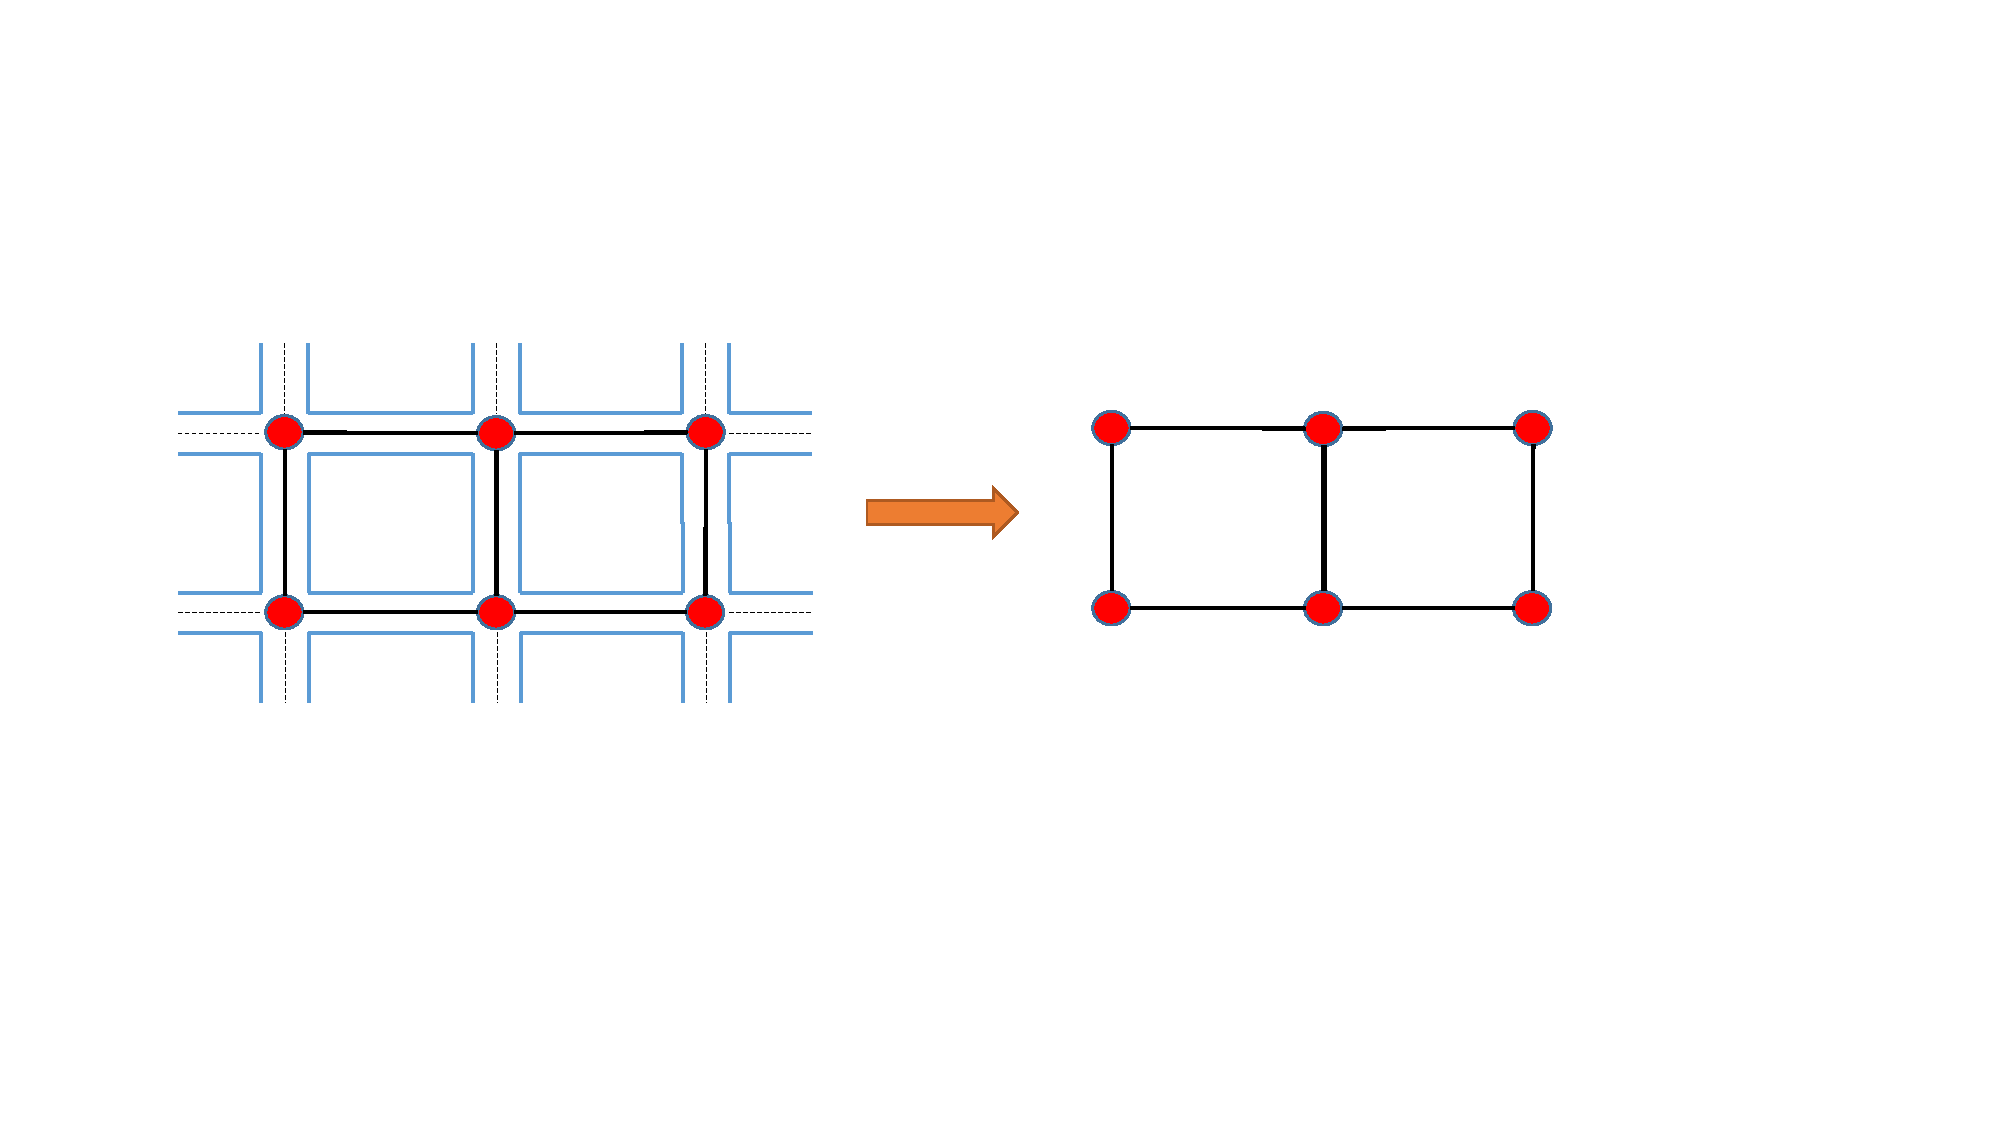
\includegraphics[width=1.2\textwidth]{ppt/network-graph.pdf}
  \caption{以路口为节点的建图方式示意图}
  \label{fig:network-graph-old}
\end{figure}
在这种建模方式下,每条车道的车辆以及当前的相位将作为该节点的特征。这种建模方式虽然可以很清晰的将多路口场景变成一张图。但是,因为是以一个路口为一个节点,所有车道的状态信息都整合到了一起,有些车道的的信息对目标节点是无用的,
如\autoref{fig:information-redundancy}所示:
\begin{figure}[htb]
  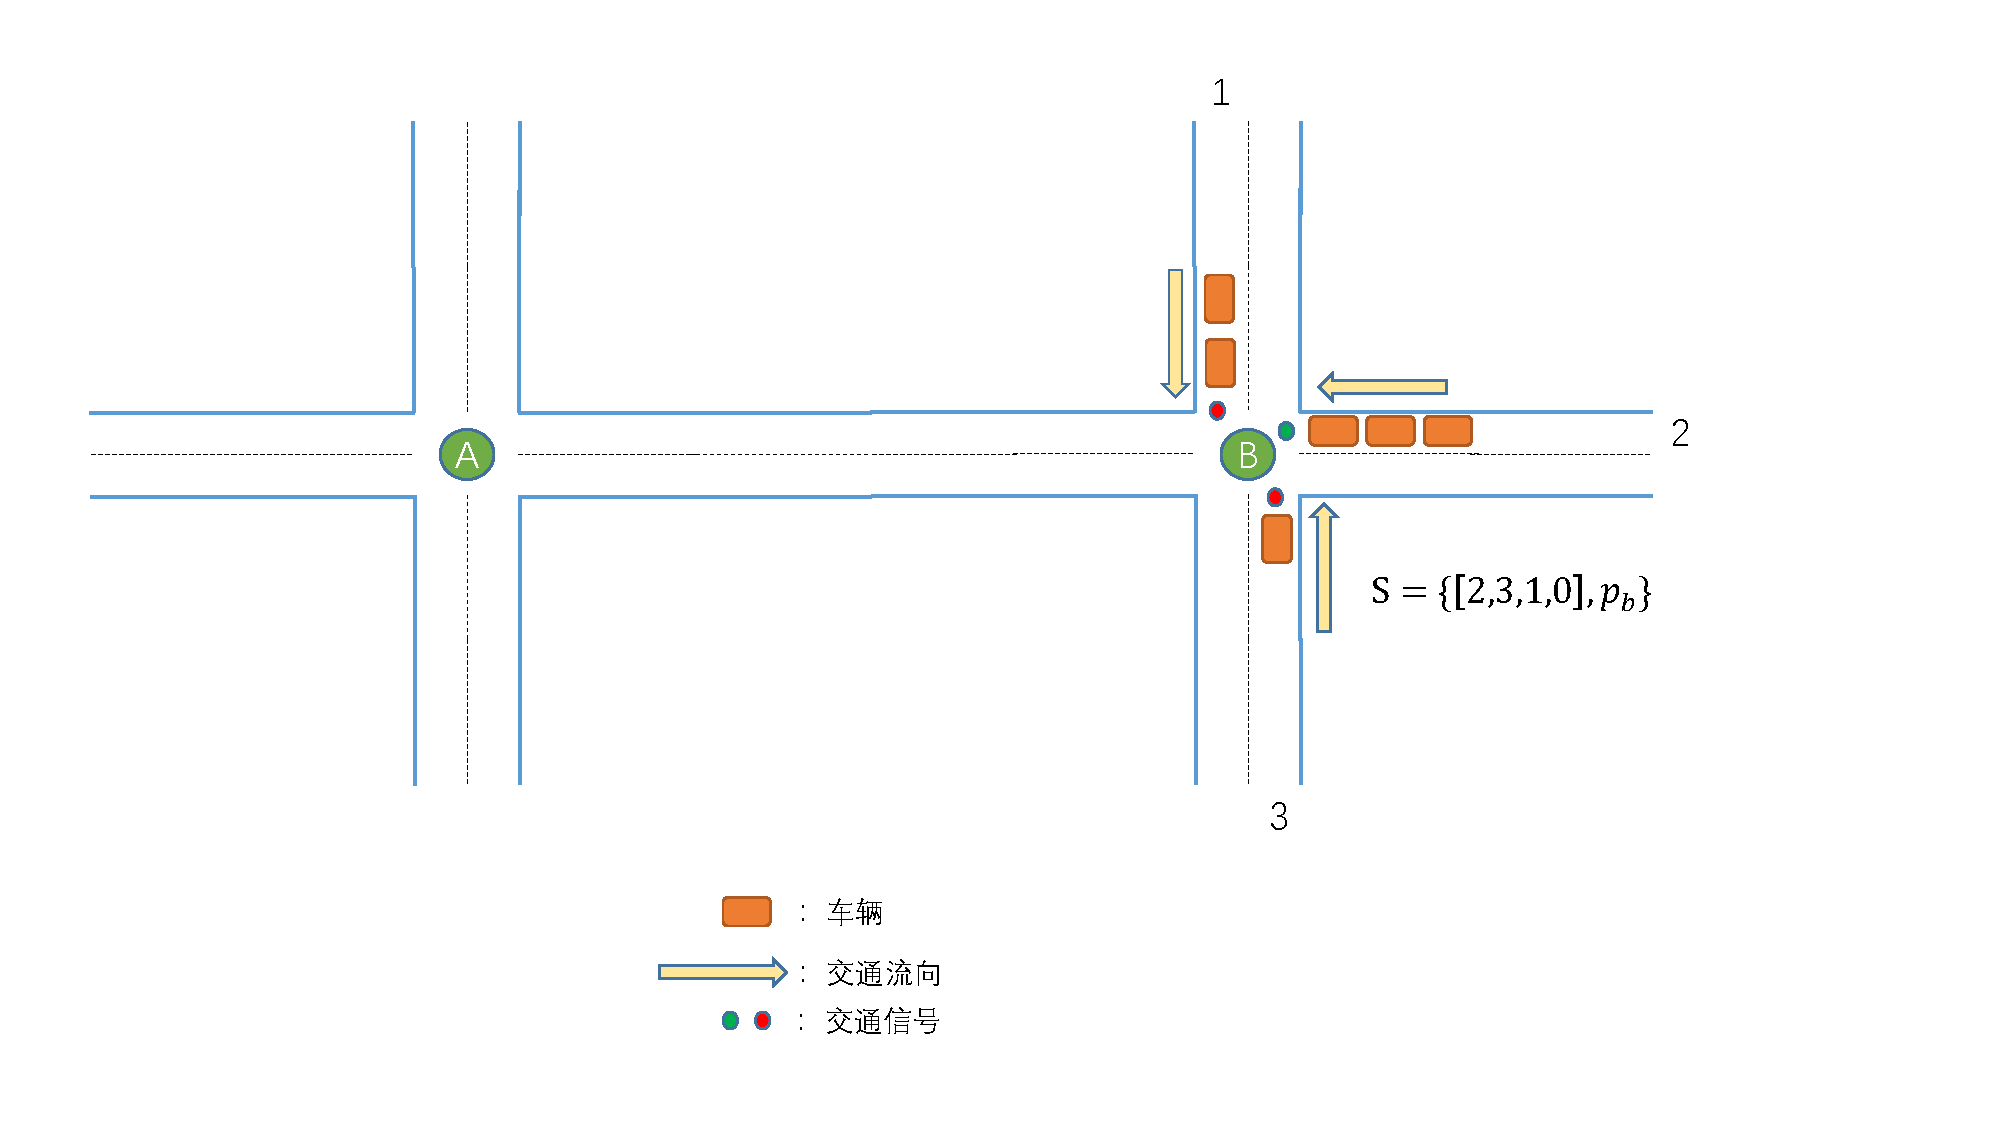
\includegraphics[width=1.2\textwidth]{ppt/information-redundancy.pdf}
  \caption{在以路口为节点的建图方式下的信息传递示意图}
  \label{fig:information-redundancy}
\end{figure}
路口B中只有2车道的交通流向与A车道有关,1、3车道的车辆不会行驶到A路口。在信息传递的时候,如果将所有的信息都笼统地传递过去,将会增加A提取有效信息的难度,从而降低学习的效率。

\section{改进}
本文同样采用IRL with Communication的框架,与已有工作不同的是,我们采用不同的建模方式:以道路为节点进行图建模,即一条道路就是一个节点,如\autoref{fig:network-graph-new}所示:
\begin{figure}[htb]
  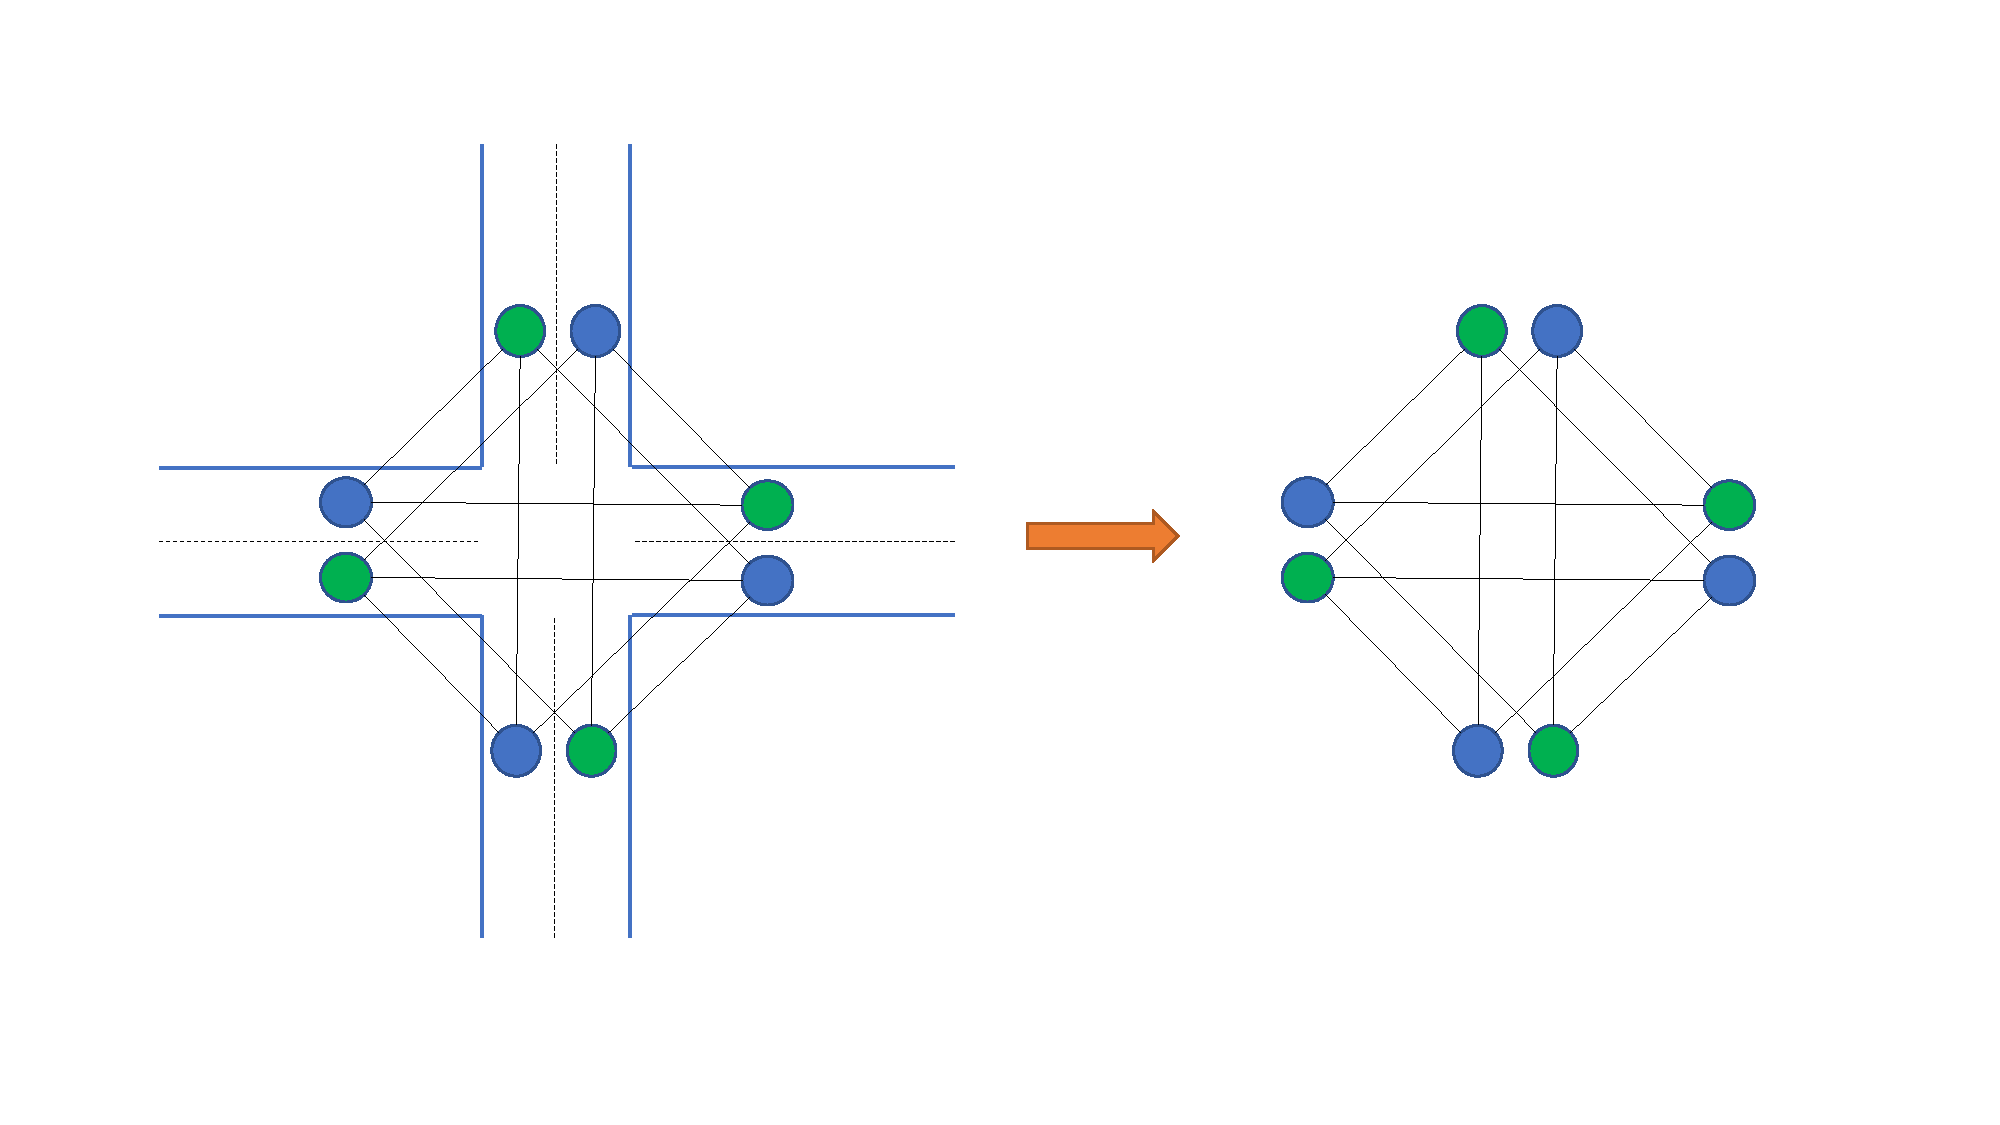
\includegraphics[width=1.2\textwidth]{ppt/graph-modeling.pdf}
  \caption{以道路为节点的建图方式示意图}
  \label{fig:network-graph-new}
\end{figure}

此外,我们根据当前的相位对图的边设一个权重。这里我们规定,如果在当前相位下,道路$i$到道路$j$之间的交通是允许通行的,则表示$(i,j)$的状态是'connected'。权重的定义方法如下:
\begin{align}
  w_{i,j} = \begin{cases}
    1 & (i, j) \text{ is connected} \\
    0 & \text{otherwise}
  \end{cases}
\end{align}
这个权重将被用于剔除对目标节点无用的信息。

这里我们沿用\inlinecite{wei2019colight,wang2020stmarl}工作使用图注意网络,但是与之不同的是,我们不是学习相邻智能体和目标智能体的隐藏状态之间的动态相互作用,而是用来做节点回归(Node Regression),即估计目标节点在下一个时间点的特征。
\section{方法}
\subsection{重要性计算}
为了了解节点$j$(源节点)的信息在确定节点$i$(目标节点)下一时刻的特征的重要性,我们首先嵌入两个节点的特征,然后计算他们之间的相关系数$e_{i j}$(节点$j$在确定节点$i$的特征时的重要性),具体操作如下:
\begin{align}
  e_{i j}=a\left(\left[W h_{i} \| W h_{j}\right]\right)
\end{align}
其中$W$是一个共享参数,用来进行特征增强,然后用$[\cdot \| \cdot]$对节点$i$和节点$j$增强后的特征进行拼接,最后使用$a(\cdot)$将拼接后的高维特征映射到一个实数上。
\subsection{特征筛选}
由于当前交通信号的影响,道路$j$的车辆不会进入到道路$i$,即节点$j$的信息在确定节点$i$的下一时刻的特征时是无用的,因此我们要筛选掉对目标节点无用的信息。这里我们通过之前介绍的边的权重来实现:
\begin{align}
  \label{eq:mul_phase}
  e_{i j} = e_{i j} * WE_{i j},
\end{align}
如果$WE_{i j} = 1$(即道路$j$到道路$i$的交通在当前相位下是可以通行的),$e_{ij}$将维持之前的计算结果。反之,如果$WE_{i j}=0$,将清除节点$j$对节点$i$的影响。
\subsection{注意力分布计算}
为了重新确定源节点和目标节点之间的注意力值,我们进一步将目标节点$i$和其邻近节点之间的交互等分进行归一化:
\begin{align}
  \alpha_{i j}=\operatorname{softmax}\left(e_{i j}\right)=\frac{\exp \left(e_{i j} / \tau\right)}{\sum_{j \in \mathcal{N}_{i}} \exp \left(e_{i j} / \tau\right)},
\end{align}
其中$\tau$是一个温度系数,$\mathcal{N}_{i}$是目标节点$i$邻近范围的节点集合。
\subsection{特征回归}
为了确定目标节点在下一个时刻的特征,这里我们将其所有邻近节点的信息按照各自的重要性进行组合:
\begin{align}
  h_{i}^{\prime}=\sigma\left(\sum_{j \in \mathcal{N}_{i}} \alpha_{i j} W h_{j}\right)
\end{align}
其中$\sigma(\cdot)$是激活函数。$h_{i}$是$i$节点融合了邻域信息后的新特征。

\subsection{Multi-Head Attention}
进一步,我们使用多头注意力机制(Multi-Head Attention)来关注不同相关性下的信息,如下所示:
\begin{align}
  h_{i}^{\prime}(K)=\sigma\left( \frac{1}{K} \sum_{k=1}^{k=K} \sum_{j \in \mathcal{N}_{i}} \alpha_{i j}^{k} W^{k} h_{j}\right)
\end{align}
其中$K$是注意力头的数量,例如当$k = 3$时,结构如图\autoref{fig:multi-head}所示:
\begin{figure}[htb]
  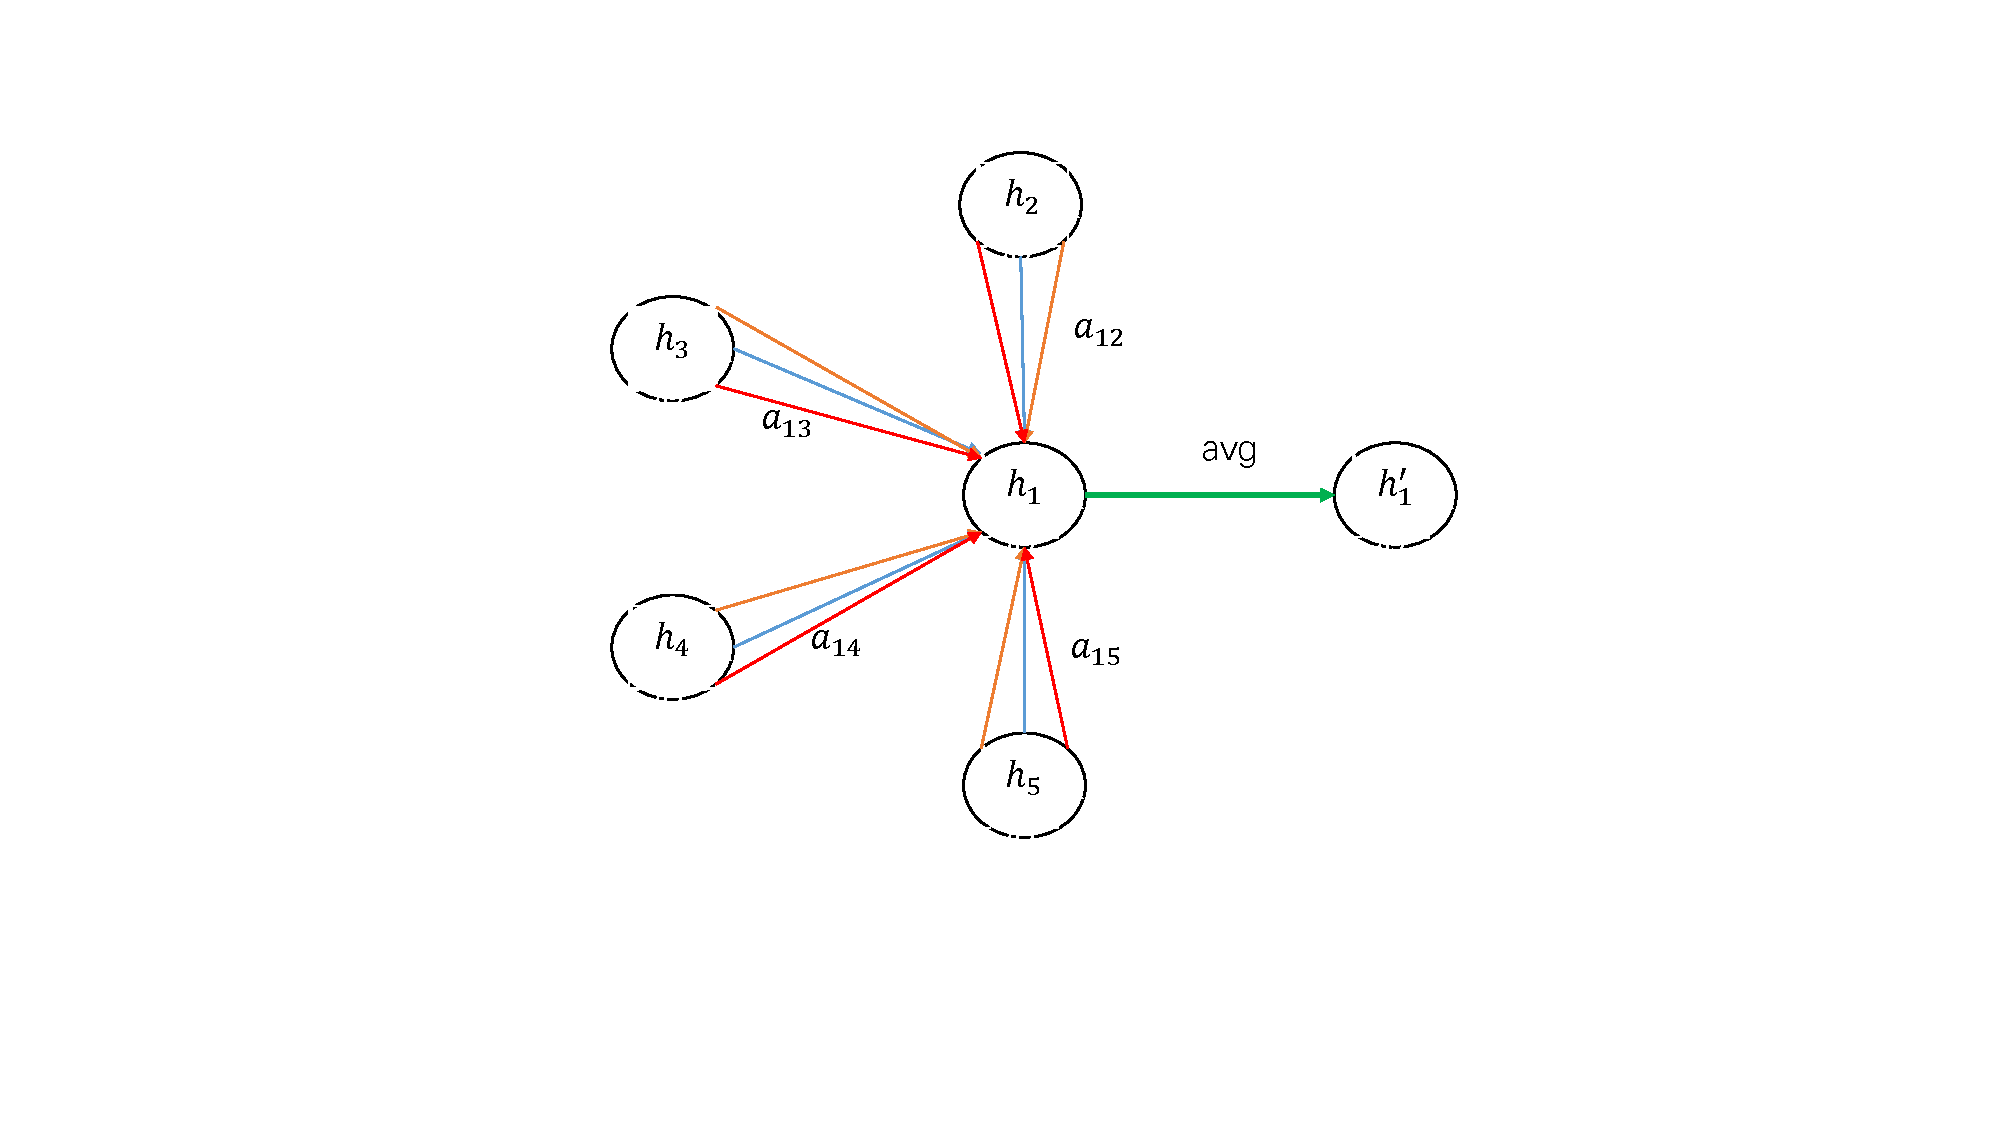
\includegraphics[width=0.9\textwidth]{fig/multi-head.pdf}
  \caption{多头注意力计算示意图($k=3$)}
  \label{fig:multi-head}
\end{figure}

对于每个路口,我们要估计每条引进道路在下一调度时刻的状态,即我们要对四个节点进行计算,如\autoref{fig:node-regression}中A路口的四个红色节点。通过在目标节点(红色节点)的及其邻近节点(绿色节点)构成的子图(如图\autoref{fig:node-regression}中右上角的图)上对目标节点进行上述的计算。
\begin{figure}[htb]
  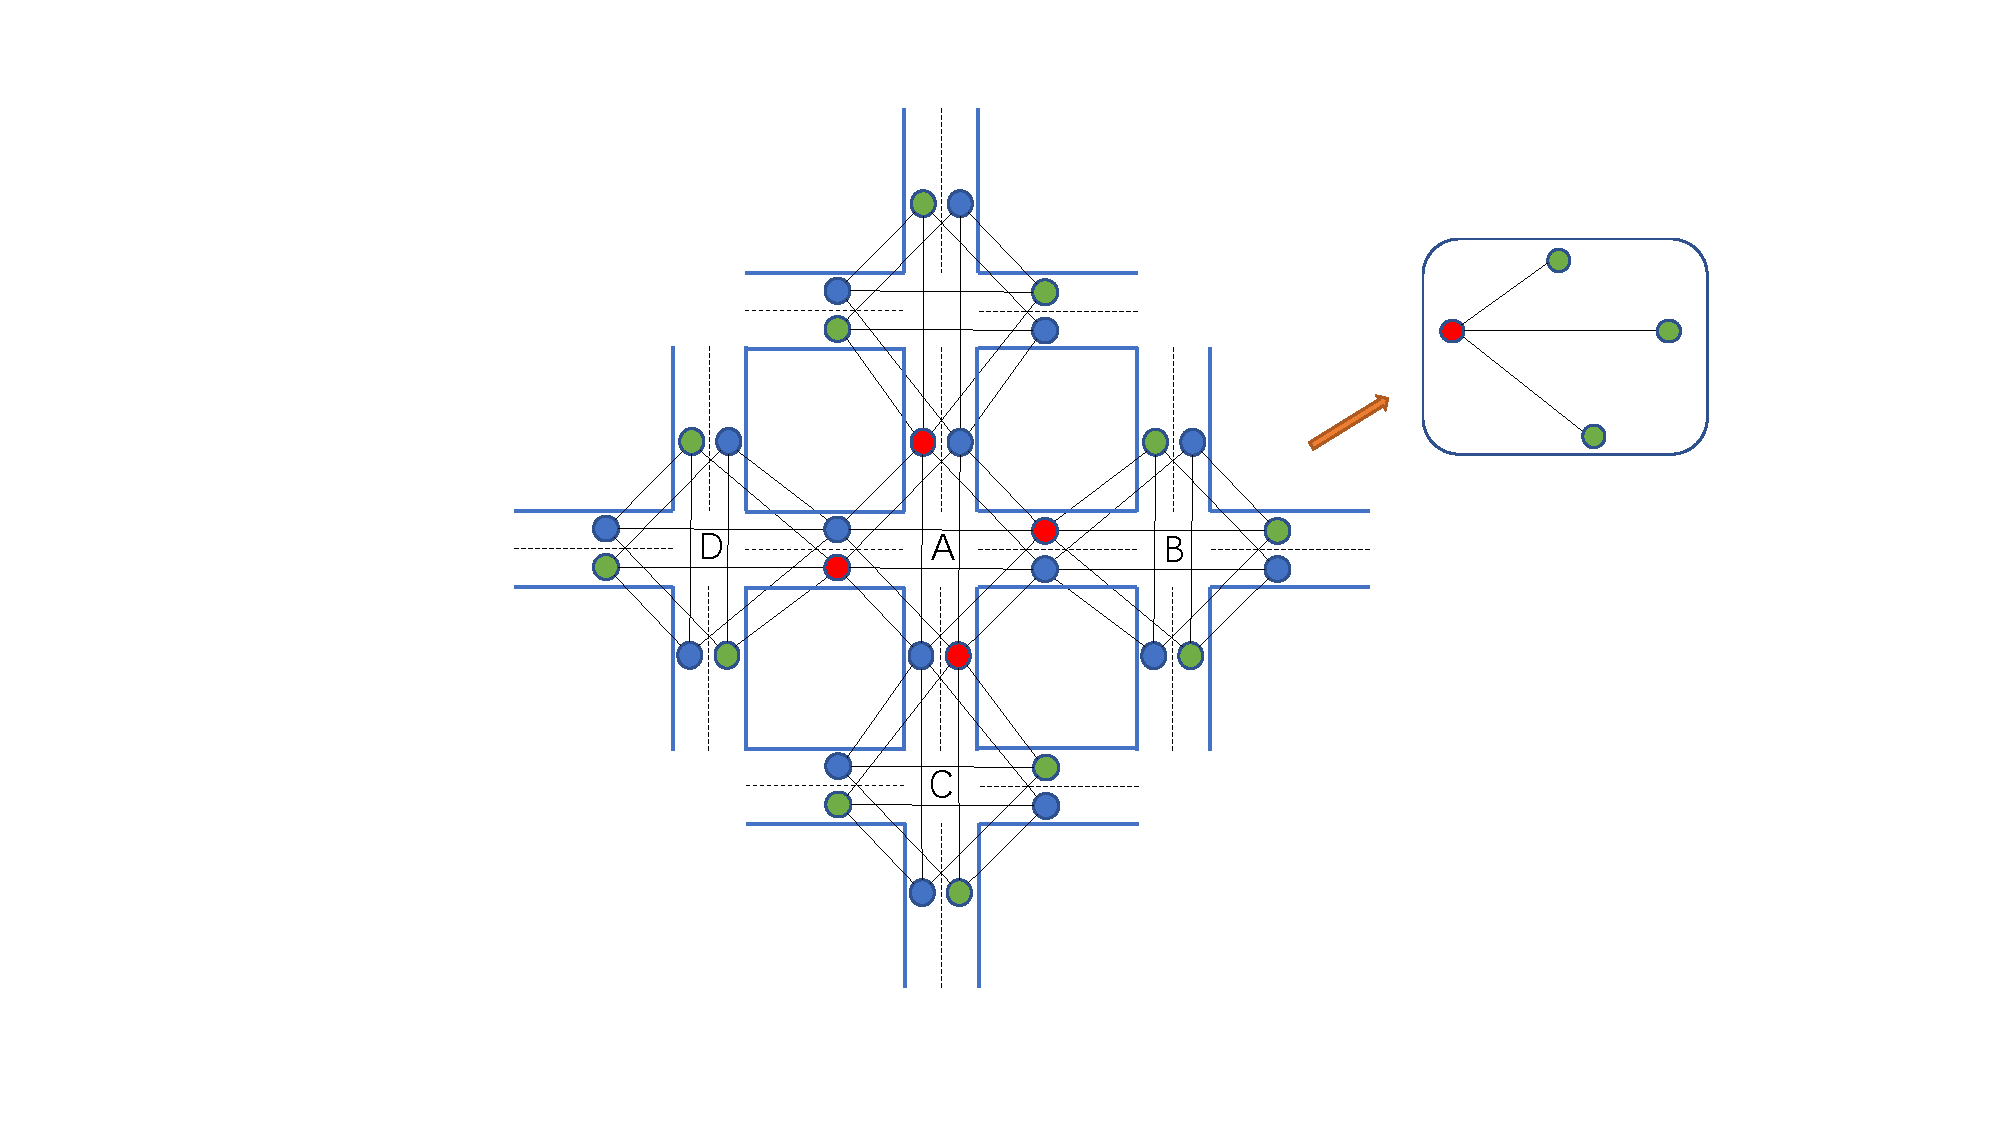
\includegraphics[width=0.9\textwidth]{fig/node-regression.pdf}
  \caption{节点回归计算示意图}
  \label{fig:node-regression}
\end{figure}
由于我们是以道路为节点进行建图的,所以即便是单个路口也可以表示成一个图,所以当有多个路口的时候,会产生一张很大的图。这里每个节点维护自己路口的子图,包括更新子图中的节点特征以及边的权重(根据当前路口的信号相位确定)。

\subsection{模型框架}
如\autoref{fig:model-framework}所示,对于单个路口来说,有两个模型,一个是用来进行交通信号控制的DQN模型$\mathcal{Q}$,另一个是用来预测下一调度时刻状态的GAT模型$\mathcal{G}$。
对于DQN模型来说,每次根据输入的状态来选择动作,其中状态由以下几部分组成:
\begin{itemize}
  \item Queue length:当前路口每条车道的队列长度。
  \item Traffic volume:当前路口每条车道的车辆数。
  \item Current Phase:路口当前的相位。
  \item Next Queue length:通过节点回归估计的下一调度时刻的Queue length。
  \item Next Traffic Volume:通过节点回归估计的下一调度时刻的Volume。
\end{itemize}
其损失函数如\autoref{eq:loss-dqn}所示:
\begin{align}
  \label{eq:loss-dqn}
  \mathcal{L}_t=[ r_{t+1}+\gamma \mathop{\arg\max}_{a^{\prime}} \mathcal{Q}(s_{t+1},a^{'};\theta)-\mathcal{Q}(s_t,a_j;\theta)]^2,
\end{align}

对于GAT模型来说,首先我们规定节点的特征$f_t=\{q_t, v_t\}$,其中$q_t$和$v_t$分别时队列长度(Queue length)和交通流量(Traffic volume)。当环境转移到新的状态$s_{t+1}$时,更新节点特征($f_{t+1}=\{q_{t+1},v_{t+1}\}$)以及边的权重,其损失函数如下所示:
\begin{align}
  \label{eq:loss-gat}
  \mathcal{L}_G = [f_{t+1} - f_{t+1}^{\prime}]^2
\end{align}
其中$f_{t+1}^{\prime}$是在$t$调度时刻,利用邻近节点信息预估的下一时刻的节点特征,是预测值,而$f_{t+1}$是$t+1$时刻的真实节点特征。

具体的算法流程如\autoref{alg:dqn-gat}所示。
\begin{breakablealgorithm}
  \caption{multi-intersection}
  \label{alg:dqn-gat}
  \begin{algorithmic}[1] %每行显示行号  
      \Require 
      $E$ : 学习片段数 \newline
      $T$ : 每个学习片段的步数 \newline
      $b$ : 学习经验数 \newline
      $\epsilon$ : 随机选择动作概率 \newline
      $\gamma$ : 折扣因子 \newline
      $\Delta t$ : 信号维持时间
      \For{$episode=1,E$}  
          \State 初始化环境。
          \For{$t=1,T$}
              \State 从环境中获取当前状态观测$s_t={q_t, v_t, p_c}$。
              \State 使用GAT估计下一调度时刻的节点特征$f_{t+1}^{\prime}=\{q_{t+1}^{\prime},v_{t+1}^{\prime}\}$。
              \State 生成一个0到1之间的随机数$rand$。
              \If{ $rand < \epsilon$}
                  \State 从动作空间中随机采样一个动作$a_t$。
              \Else
                  \State 使用DQN模型选择动作:$a_t = \mathop{\arg\max}_a \mathcal{Q}((s_t||f_{t+1}^{\prime}),a;\theta)$。
              \EndIf
              \State 将当前信号更改为$a_t$并维持$\delta t$秒时间。
              \State 环境转移到新的状态$s_{t+1}$并返回一个奖励$r_{t+1}$。
              \State 更新节点特征$f_{t+1}={q_{t+1}, v_{t+1}}$。
              \State 计算GAT损失函数$\mathcal{L}_G$:
              $\mathcal{L}_G = [f_{t+1} - f_{t+1}^{\prime}]^2$
              \State 更新GAT模型参数。
              \State 将经验$(s_t,a_t,r_{t+1},s_{t+1})$ 存储到经验回放池M中。
              \If{$|M|>b$}{
                  \State 从经验回放池M中随机采样b条经验数据。
                  \State 计算DQN损失函数 $\mathcal{L}_Q$:
                  $\mathcal{L}_Q=[ r_{t+1}+\gamma \mathop{\arg\max}_{a^{\prime}} \mathcal{Q}(s_{t+1},a^{\prime};\theta)-\mathcal{Q}(s_t,a_t;\theta)]^2$;
                  \State 更新DQN模型参数。
              }
              \EndIf
          \EndFor
      \EndFor  
  \end{algorithmic}  
\end{breakablealgorithm}  

\begin{figure}[htb]
  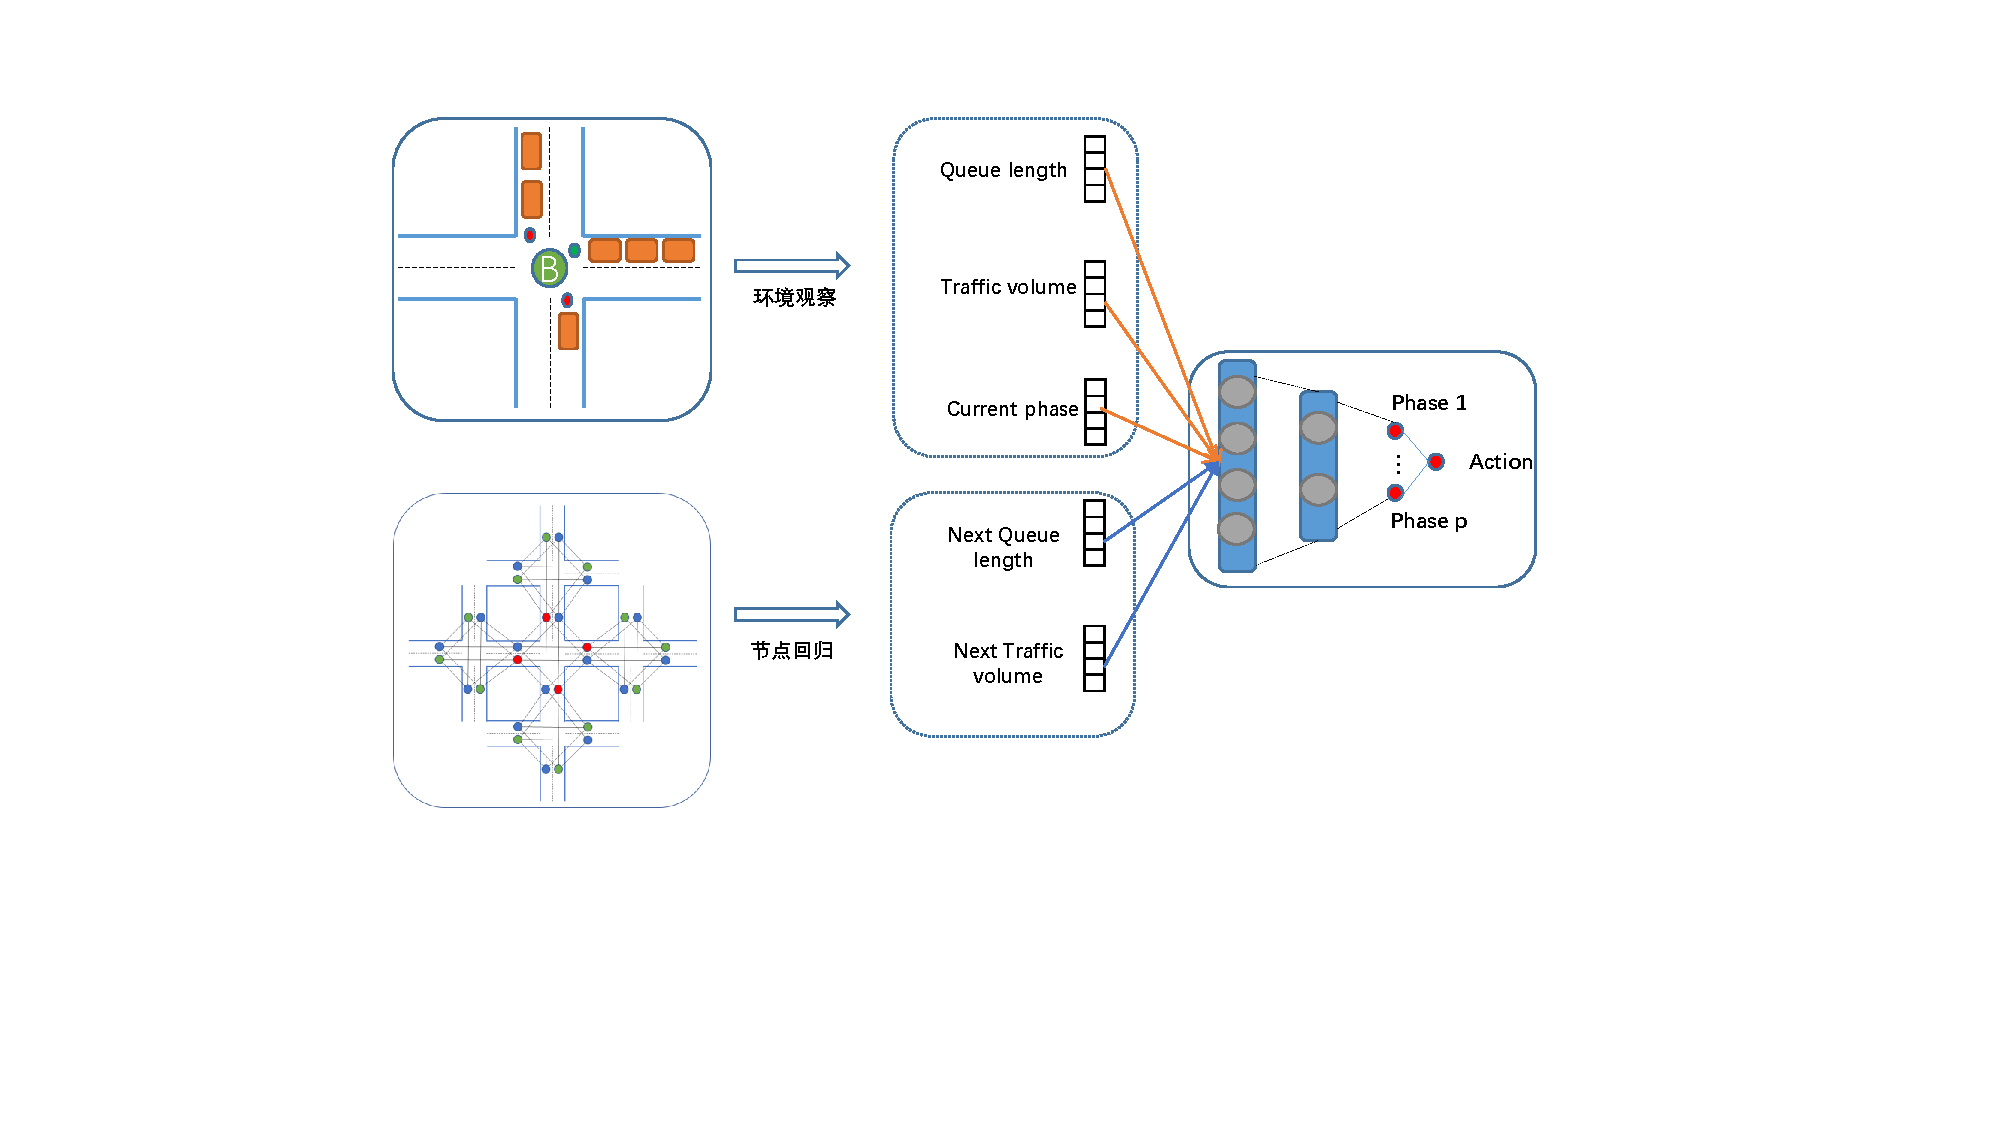
\includegraphics[width=1.4\textwidth]{fig/model-framework.pdf}
  \caption{模型框架}
  \label{fig:model-framework}
\end{figure}
\section{实验}
我们在三个合成的数据集以及两个真实数据集上对我们的方法进行了实验,以评估我们方法的性能。由于实验是针对大规模的多路口场景,我们这里的仿真工具使用的是CityFlow\footnote{http://cityflow-project.github.io},其对大规模交通信号控制的支持更加出色。
\subsection{数据集介绍}

\textbf{合成数据:}延用\inlinecite{wei2019colight}的做法,我们在不同的道路($Arterial_{1\times3}$, $Grid_{3\times3}$, $Grid_{6\times6}$)上中使用了两种合成数据,即单向交通和双向交通。
% 在合成道路网中,每个路口有四个方向(西\rightarrow东、东\rightarrow西、南\rightarrow北以及由北\rightarrow南),每个方向有三条车道,每条车道长300米,宽3米。

\textbf{真实数据:}我们还使用了杭州和济南两个城市某个路段下采集到的真实数据\footnote{https://traffic-signal-control.github.io/\#open-datasets}进行了实验,\autoref{tab:real-world-datasets}统计了这两个数据集的关键信息。
\begin{table}[htb]
  \caption{数据统计}
  \label{tab:real-world-datasets}
  \begin{tabular}{lccccc}
  \toprule
  \multirow{2}{*}{数据集} & \multirow{2}{*}{路口数量} & \multicolumn{4}{c}{车辆到达率(300辆/s)} \\
  & & \multicolumn{1}{c}{均值} & \multicolumn{1}{c}{方差} & \multicolumn{1}{c}{最大值} & \multicolumn{1}{c}{最小值} \\
  \midrule
  $D_{Hangzhou}$ & 16 & 526.63 & 86.70 & 676 & 256 \\
  $D_{Jinan}$ & 12 & 250.70 & 38.21 & 335 & 208 \\
  \bottomrule
  \end{tabular}
\end{table}
\begin{itemize}
  \item $D_{Hangzhou}$:这个数据集中有16个路口,其中交通数据是由路侧监控摄像头拍摄产生,每条数据包含时间、摄像头ID和车辆信息。通过使用摄像头位置分析这些记录,记录车辆通过道路交叉口时的轨迹。我们以通过这些路口的车辆数作为实验的交通量。
  \item $D_{Jinan}$:与$D_{Hangzhou}$类似,数据集中包含了12个路口。
\end{itemize}:

\subsubsection{比较方法}
我们将我们的方法与传统交通控制方法和基于强化学习的几种方法进行了对比:
\begin{itemize}
  \item FT\cite{koonce2008traffic}: 这种方法以预先设定的方式循环改变信号。
  \item MaxPressure\cite{varaiya2013max}:交通领域最先进的网络级的交通信号控制方法,每次调度时,选择压力最大的相位。
  \item Individual RL\cite{wei2018intellilight}:一种基于深度强化学习的交通信号控制方法,不考虑邻居信息。每个路口由一个智能体控制,智能体之间不共享参数,而是独立更新自己的网络。
  \item GCN\cite{van2016coordinated}:一种基于深度强化学习的交通信号控制方法,使用图卷积神经网络(GCN)提取相邻路口的交通特征,不过其图建模方式是以路口为节点。
  \item Colight\cite{wei2019colight}:与GCN方法类似,都是以路口为节点的图建模方法,不过其使用GAT来学习不同路口之间的动态交互。
  \item GAT-Road:我们的方法,基于一种新的图建模方式(以道路为节点)。
\end{itemize}
\subsubsection{性能表现}

\begin{table}[htb]
  \caption{不同方法在合成数据集和真实数据集上关于平均通行时间的表现}
  \label{tab:performance}
  \begin{tabular}{lcccc}
  \toprule
  方法 & $Grid_{6x6}-Uni$ & $Grid_{6x6}-Bi$ & $D_Hangzhou$ & $D_Jinan$ \\
  \hline
  Fixedtime & 209.68 & 209.68 & 728.79 & 869.85 \\
  MaxPressure & 186.07 & 194.96 &  422.15 & 361.33 \\
  \hline
  Individual RL & 314.82 & 261.60 & 345.00 & 325.56 \\
  GCN & 205.40 & 272.14 & 768.43 & 625.66 \\
  CoLight & 173.79 & 170.11 & 297.26 & 291.14 \\
  \hline
  GAT-Road & \textbf{156.32} & \textbf{161.56} & \textbf{290.44} & \textbf{279.67} \\
  \bottomrule
  \end{tabular}
\end{table}
我们在合成数据和真实数据上进行了大量实验,并和已有方法进行了对比,然后在通行效率和模型收敛性上进行了分析。

\subsubsection{性能比较}

\textbf{效率比较}:
\autoref{tab:performance}列出了所有方法在合成数据和真实数据上路口的平均通行时间,可以看出,无论是在合成数据还是真实数据集上,我们的方法都取得了最好的表现。进一步的观察数据可以看出:
与传统交通控制中最先进的方法(MaxPressure)相比,我们的方法在合成数据和真实数据上都取得了一致的性能改进,其中在合成数据上的平均改进率是$16.6\%$,在真实数据上的平均改进率是$26.9\%$。

在合成数据上,Fixedtime的表现相对比较出色,但是在真实数据上,和基于学习的方法的性能差异变得明显。这是因为人为合成的数据是相对比较规则的数据,车辆流动的随机性没有真实数据中强,交通相对更加稳定。

GCN在真实数据上的表现并不出色是因为其在经行Communication时,是根据预先定义的静态重要性处理邻居节点的信息,而不是根据实时的交通情况进行动态调整。


\textbf{收敛性比较}
\begin{figure}[t]
  \label{fig:convergence}
  \subfloat[$Grid_{6x6}$]{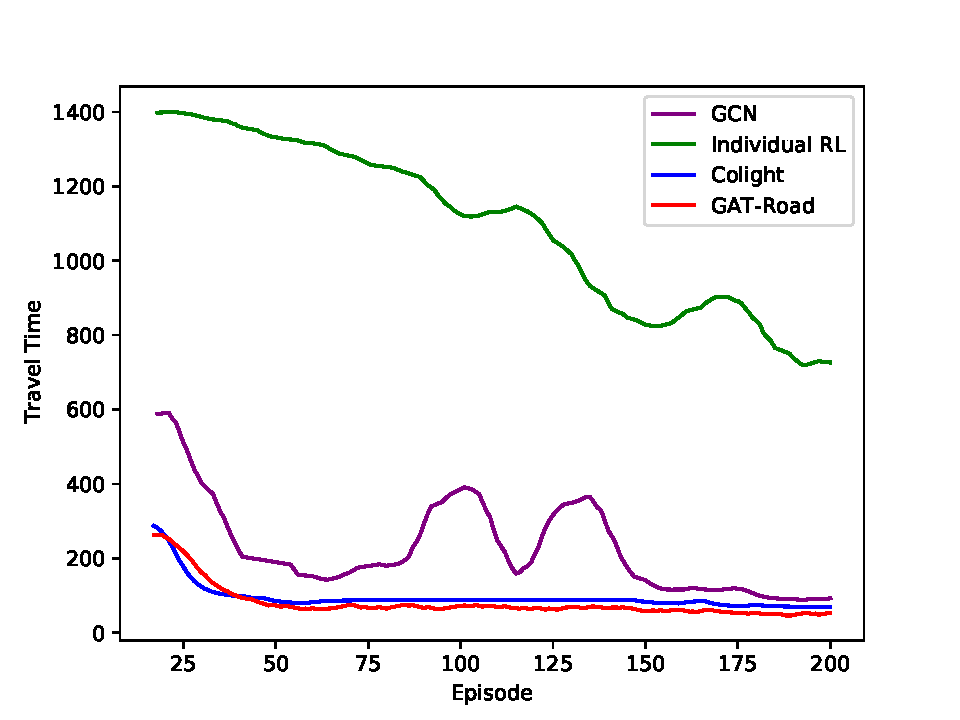
\includegraphics[width=0.45\textwidth]{./fig/conv-6x6.pdf}}\quad
  \subfloat[$Grid_{6x6}$-b]{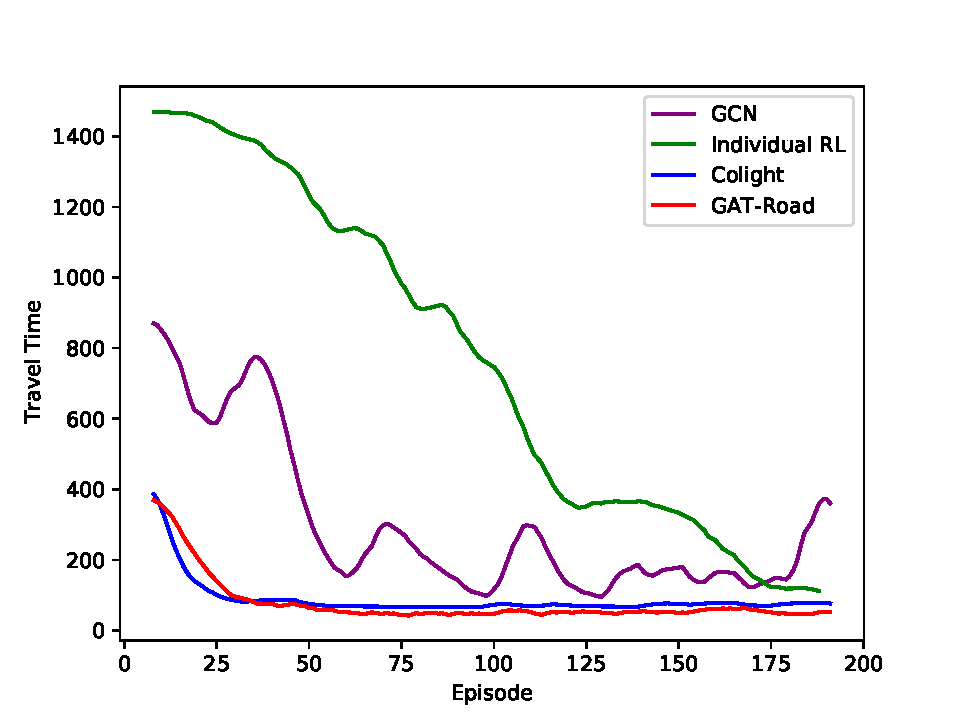
\includegraphics[width=0.45\textwidth]{./fig/conv-6x6-b.pdf}}\\
  \subfloat[$D_{Hangzhou}$]{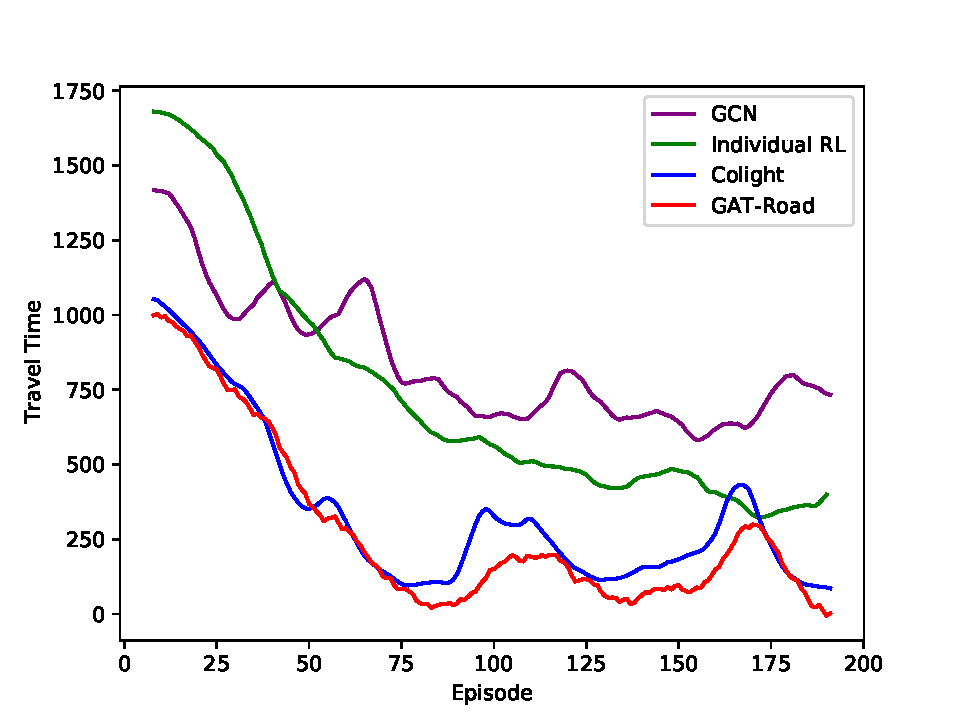
\includegraphics[width=0.45\textwidth]{./fig/conv-Hangzhou.pdf}}\quad
  \subfloat[$D_{Jinan}$]{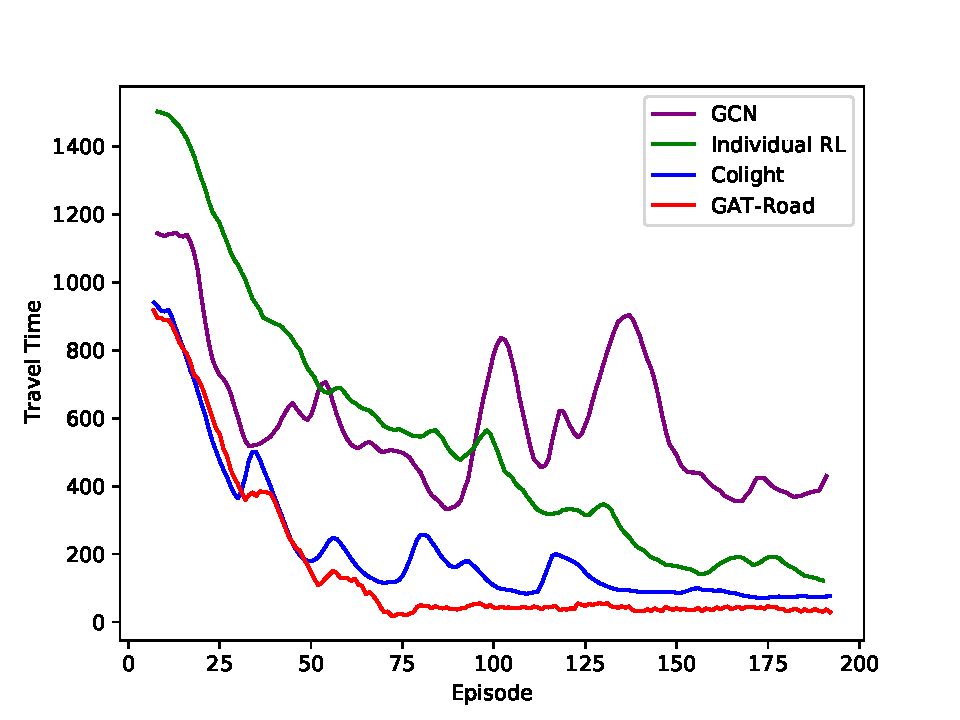
\includegraphics[width=0.45\textwidth]{./fig/conv-Jinan.pdf}}
  \caption[]{GAT-Road和其他三种基于学习的方法的收敛速度}
\end{figure}

我们将GAT-Road与其他三种基于学习的方法在不同数据上的学习收敛速度进行了比较,结果如\autoref{fig:convergence}所示。

与同样是使用IRL with Communication框架的GCN和Colight相比,我们的方法的收敛速度更快,这得益于我们提出的新的建图方式,在这种建图方式下,节点在进行信息聚合时可以剔除与目标节点无关的信息,从而降低了学习的难度,模型更容易收敛。

虽然Individual最终也能收敛到最佳性能,但是由于其是独立优化单个路口的策略,没有考虑到周围路口环境的交通信息,因此其刚开始时的性能表现相较于其他三种方法更差,并且收敛速度更慢。
